%Tema para beamer "CCM1" versión 1
%Desarrollo por Erick David Luna Núñez y 
%Fernanda Barajas Hernandez

\documentclass{beamer}

\usepackage[utf8]{inputenc}
\usepackage{heuristica}
\usepackage[T1]{fontenc}
\usepackage[heuristica,vvarbb,bigdelims]{newtxmath}
\renewcommand*\oldstylenums[1]{\textosf{#1}}
\usepackage[sfdefault,scaled=.85]{FiraSans}
\usepackage{graphicx}
\usepackage[spanish]{babel} 
\usepackage[pages=some]{background}
\usepackage{listings}
\usepackage{xcolor}
\usepackage{subfig}
\usepackage{multicol}
\usepackage[export]{adjustbox}

\lstdefinestyle{Bash}
{language=bash,
keywordstyle=\color{blue},
basicstyle=\ttfamily,
morekeywords={name@desktop:},
alsoletter={$\sim \$$},
morekeywords=[2]{name@desktop:},
keywordstyle=[2]{\color{blue}},
literate={\$}{{\textcolor{green}{\$}}}1 
         {:}{{\textcolor{green}{:}}}1
         {~}{{\textcolor{green}{\textasciitilde}}}1,
}
\lstset{ %Formatting for code in appendix
    basicstyle=\footnotesize,
    numbers=left,
    stepnumber=1,
    showstringspaces=false,
    tabsize=1,
    breaklines=true,
    breakatwhitespace=false,
}


\pagenumbering{arabic}

%%Se define el "environment" teorema
\newtheorem{teorema}{Teorema}

%Definir el autor con el estilo definido (el textbf y el uso del color son herramientas del diseño, no necesario borrar)
\title{\textbf{Git Essentials} \\ Curso de Inicio}

%Nombre del autor
\author{Ing. Paola B. Torres y Esp. Ing. Daniela Armijo} 

%Fecha o evento en que se presentará la plática
\date{30/06 y 07/07} 

%correo del expositor o incluir posibles colaboradores
% \institute{fulano@matmor.unam.mx} 

%%Tema de beamer "CCM-1"
\usetheme{ccm1}




\begin{document}
%Define el fondo de la primer diapositiva
{%Inicia el cambio de fondo para la portada
\setbeamertemplate{background}{%

\includegraphics[width=\the\paperwidth]{images/FONDO_AL_15.png}
}
%lo anterior es para definir el fondo de la primer diapositiva

\begin{frame}
  \titlepage %Necesario para generar la portada
\end{frame}
}%aquí termina el cambio de fondo

% \begin{frame}
% \tableofcontents %Imprime la tabla de contenido
% \end{frame}


\AtBeginSection[]
{
  \begin{frame}
    \tableofcontents[currentsection]
  \end{frame}
  % \begin{frame}
  %   \begin{structureenv}
  %   \LARGE Sección \thesection 
  %   \rule[-.6cm]{2pt}{1.5cm}
  %   \insertsection
  %   \end{structureenv}
  %   \end{frame}


  }


%%%%%%%%%%%%%%%%%%%%%%%%%%%%%%%%%%%%%%%%%%%%%%%%%%%%%%%%%%%%%%%%%%%%%%%%%%%%%%%%%%%%%


\section{Introducción} 

\subsection{¿Qué es Git?}

\begin{frame}{¿Qué es Git?}

  \begin{figure}
    \includegraphics<1->[width=0.8\textwidth]{images/cap-one.png}
    \llap {\includegraphics<2->[width=0.8\textwidth]{images/cap-two.png}}
  \end{figure}


\end{frame}


\begin{frame}{¿Qué es Git?}
  \begin{figure}
    
\includegraphics[width = 0.3\textwidth]{images/logo_git.png}
  \end{figure}

  \begin{itemize}
    \item Es una herramienta de control de versiones distribuido
    \item Permite trabajar en un proyecto sin necesidad de estar
    conectados a un servidor central.
    \item Un sistema de control de versiones es una herramienta que se utiliza para mantener un registro de los cambios que se hacen en un proyecto
    \item Documentación: \href{https://git-scm.com}{Web oficial git} 
  \end{itemize}

\end{frame}

% \subsection{¿Por qué es importante Git?} 

% \begin{frame}
%   \frametitle{¿Por qué es importante Git?} 
%   \begin{itemize}
%     \item Es un sistema distribuido.
%     \item Permite trabajar sin conexión a internet y facilita la colaboración en equipos remotos.
%     \item Gestión eficiente de modificaciones y ramas 
%     \item Facilita la incorporación de nuevas funcionalidades y la corrección de errores mediante el uso de ramas (branch)
%     \item Comparación de versiones y fusion de ramas.
%     \item Git es una herramienta open source
%   \end{itemize}
  
% \end{frame}


\begin{frame}{Centralizado vs Distribuido }

  \begin{figure}
    \subfloat[\centering]{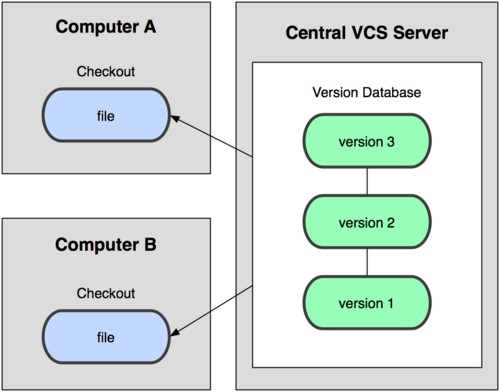
\includegraphics[width = 0.4\textwidth]{images/git-central.png}}
    \qquad
    \subfloat[\centering]{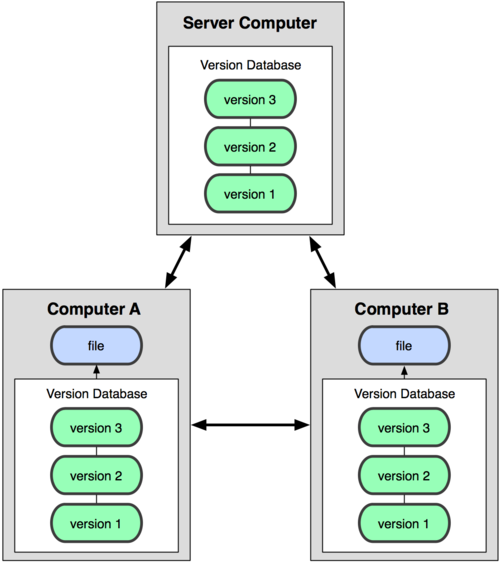
\includegraphics[width = 0.4\textwidth]{images/git-distrib.png}}
  \end{figure}

\end{frame}


\subsection{¿Cómo funciona Git?} 

\begin{frame}
  \frametitle{¿Cómo funciona Git?} 

  \begin{figure}
    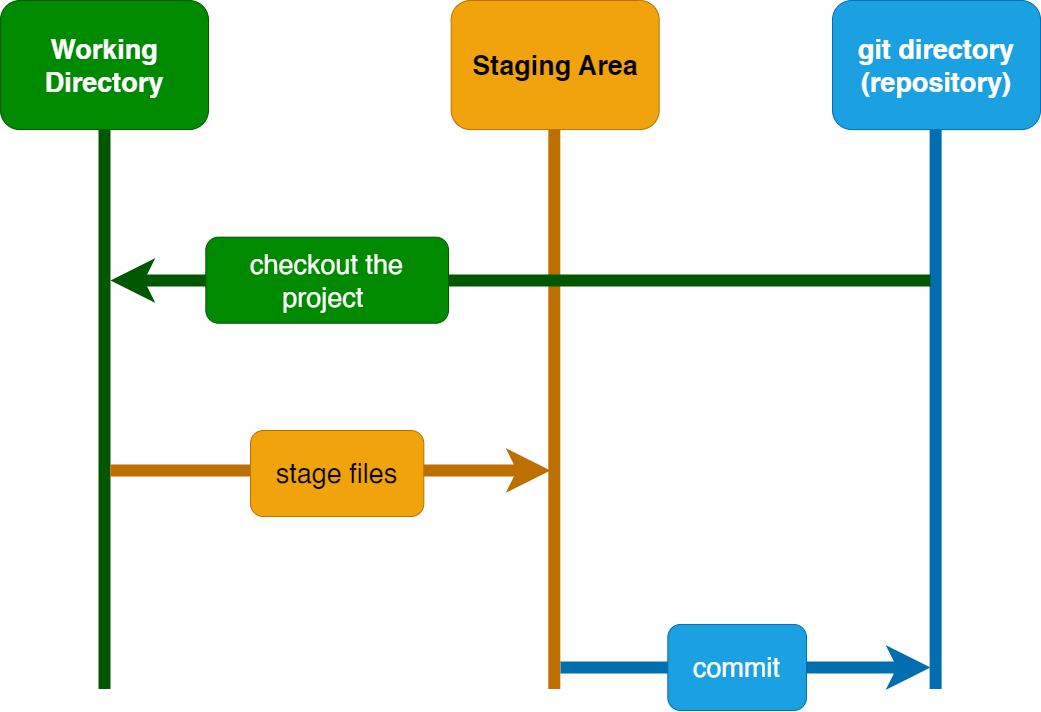
\includegraphics[width = 0.8\textwidth]{images/git-states.png}
  \end{figure}
  
\end{frame}


\begin{frame}{Plataformas} 
 
  \begin{figure}
    
\includegraphics[width=0.2\textwidth]{images/logo_github.png}
  \end{figure}

  \begin{figure}
    
\includegraphics[width=0.3\textwidth]{images/logo_gitlab.png}
  \end{figure}

  \begin{figure}
    
\includegraphics[width=0.4\textwidth]{images/logo_Bitbucket.png}
  \end{figure}
 
\end{frame}

\subsection{¿Cómo se relaciona Git con GitHub u otros servicios?} 

\begin{frame}{¿Cómo se relaciona Git con GitHub?} 


  \begin{columns}
    \begin{column}{.6\textwidth}

      \begin{itemize}

        \item Es una plataforma de alojamiento de código en la nube que utiliza el \textbf{sistema de control de versiones Git}.
        \item Colaboración en proyectos privados y abiertos. 
        \item Herramientas adicionales: seguimiento de problemas, integración continua, revisión de código y colaboración en proyectos de código abierto.
      \end{itemize}
      
    \end{column}

    \begin{column}{.4\textwidth}
      \begin{figure}
        
\includegraphics[width=0.8\textwidth]{images/logo_github.png}
      \end{figure}
    \end{column}

  \end{columns}
  

\end{frame}





% \section{Instalación y configuración}
% \subsection{¿Cómo se instala Git?}
%   \begin{frame}{¿Cómo se instala Git?} %%Otra forma (más corta) de poner el título a la diapositiva
%   \end{frame}
 
% \subsection{Creación de una cuenta en GitHub}
%   \begin{frame}{Creación de una cuenta en GitHub o un servicio de alojamiento en la nube} %%Otra forma (más 
 
%   \end{frame}
  

\section{Comandos básicos}

\subsection {Comandos útiles de terminal (bash)}

\begin{frame}[containsverbatim]{Comandos utiles de terminal}

  \begin{block}{}
    \texttt{\$ ls \\
    \$ cd <directorio>  \\ 
    \$ cd .. \\ 
    \$ pwd \\
    \$ clear  \\ 
    \$ mkdir <nombre\_directorio> \\ 
    \$ touch <nombre\_archivo>\\ 
    \$ rm <nombre\_archivo> \\ 
    \$ mv <nombre\_archivo> <directorio> \\
    \$ cp <nombre\_archivo> <directorio>}
  \end{block}

\end{frame}

\begin{frame}{Editores de Codigo}
  
\begin{columns}
  \begin{column}{0.4\textwidth}
    \begin{itemize}
      \LARGE
      \item \href{https://code.visualstudio.com/}{VS Code}
      \item \href{https://notepad-plus-plus.org/downloads/v8.5.4/}{NotePadd++} 
      \item VIM 
    \end{itemize}
  \end{column}
  \begin{column}{0.5\textwidth}
  \begin{figure}
    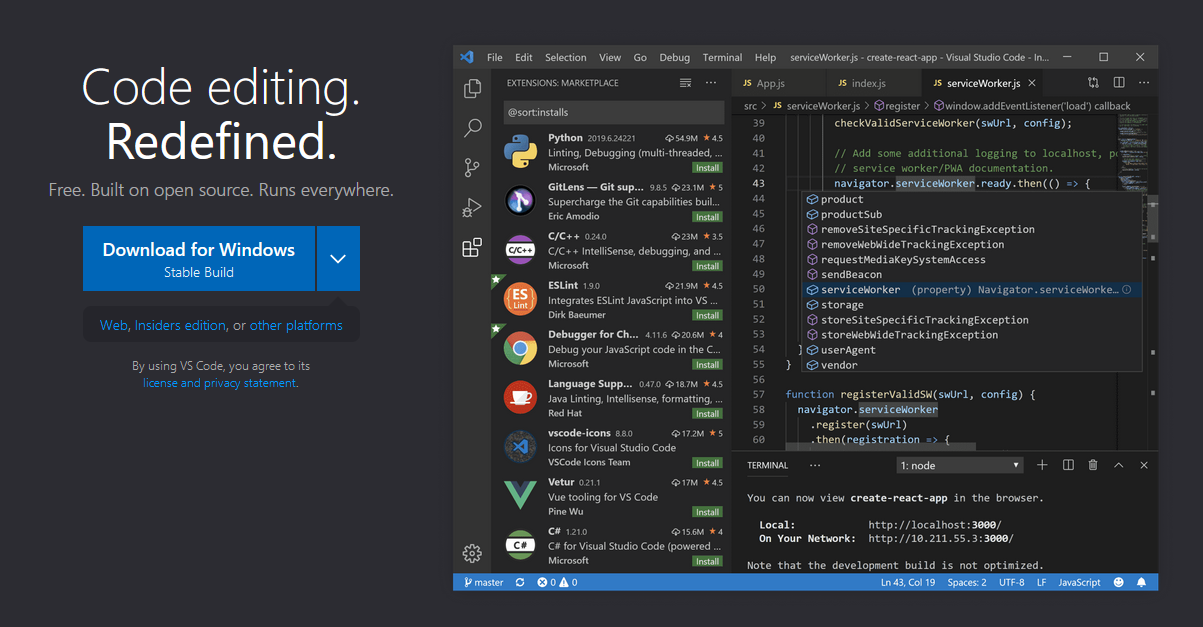
\includegraphics[width=1.2\textwidth]{images/vscode.png}
  \end{figure}
  \end{column}
\end{columns}


\end{frame}



\subsection{ Configuración básica de Git}
  
  \begin{frame}[containsverbatim]{Configuración básica de Git} 
  
    \begin{block} {}
    {\texttt {git config }} \\ 
    {\texttt {git config --global user.name <nombre>}} \\ 
    {\texttt {git config --global user.email <email>  }}
    \end{block}

  Ref: Documentación \href{https://docs.github.com/es/get-started/getting-started-with-git/setting-your-username-in-gits}{git config }
  \end{frame}
 
\subsection {Creación de un repositorio Git}
  
\begin{frame}[containsverbatim]{Creación de un repositorio desde GitHub}

\begin{block}{Crear un repositorio en GitHub}
  Vamos a \href{https://github.com}{GitHub} 
\end{block}


\begin{block}{Clonar un repositorio desde GitHub: HTTPS}
  \small
  \texttt{git clone https://github.com/user/repositorio.git .}
\end{block}

\begin{block}{Clonar un repositorio desde GitHub: SSH}
  \small
  \texttt{git clone git@github.com:/user/repositorio.git .}
\end{block}

Ref: Documentación para \href{https://docs.github.com/es/authentication/connecting-to-github-with-ssh/about-ssh}{autenticación ssh}

\end{frame}


\begin{frame}[containsverbatim] {Creación de un repositorio Git}  

\begin{block}{}

  \texttt{mkdir <nombre\_carpeta>} \\ 
  \texttt{git init}

\end{block}

\begin{block}{Conectar repositorio a la nube de GitHub}
  \small 
  \texttt{git remote add origin git@github.com:user/repositorio.git} \\ 
  \texttt{git branch -M \textbf{main}} \\
  \texttt{git push -u origin \textbf{main}}

\end{block}


\end{frame}

\subsection {Gestión de archivos}

\begin{frame} {Gestión de archivos}

  \begin{block}{Agregar archivos }
    {\texttt{\$ git add <nombre\_archivo> }}
  \end{block}

  \begin{block}{Mover archivos}
    \texttt{\$ git mv <nombre\_archivo>}
  \end{block}

  \begin{block}{Elimnar archivos}
    \texttt{\$ git rm <nombre\_archivo>}
  \end{block}

\end{frame}


\subsection {Confirmar cambios en el repositorio}

  \begin{frame} {Confirmar cambios en el repositorio}

    \begin{block}{Primero: Agregar archivos }
      {\texttt{\$ git add [archivo] }}
    \end{block}

    \begin{block}{Segundo: git commit}
      {\texttt{\$ git commit -m `insertar mensaje simple y preciso' }}
    \end{block}

    \begin{block}{Tercero: git push}
      {\texttt{\$ git push}}
    \end{block}

  \end{frame}


  \subsection {Historial de cambios y estado del repositorio}

  \begin{frame} {\LARGE Historial de cambios y estado del repositorio}
    
    \begin{block}{Estado de los archivos}
      {\texttt{\$ git status}} 
    \end{block}

    \begin{block}{Historial}
      {\texttt{\$ git log}} \\
      \texttt{\$ git log --pretty=oneline} \\
      \texttt{\$ git log --graph} \\ 
    \end{block}


  \end{frame}


\subsection{Hash: identificador de commits}

\begin{frame}

  \begin{alertblock}{¿Qué es un Hash?}
    Una función criptográfica hash es un algoritmo matemático que transforma cualquier bloque arbitrario de datos en una nueva serie de caracteres con una longitud fija (40 caracteres)
    \end{alertblock}  

\begin{figure}
  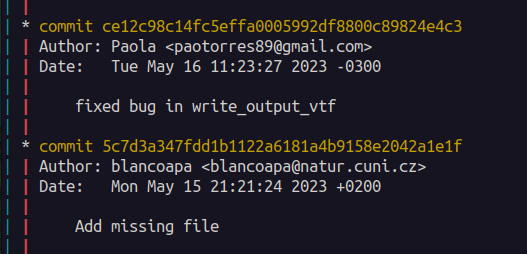
\includegraphics[width=\textwidth]{images/git-hash.png}
\end{figure}


\end{frame}


\begin{frame}{Bifurcación }

    \begin{block}{Fork (bifurcación)}
      Permite copiar un repositorio en nuestro GitHub para poder realizar cambios en un repositorio publico para el cual no tenemos permisos.
      \begin{figure}
        
\includegraphics[width=\textwidth]{images/git-fork.PNG}
      \end{figure}
    \end{block}

  \end{frame}

  \begin{frame}{Pull request}


  \end{frame}

\begin{frame}{\LARGE Práctica}
  
  \begin{alertblock}{}

    Añadir su nombre de usuario de GitHub al final del archivo \texttt{welcome.md} que se encuentra en el repositorio original del curso, mediante un \texttt{pull request}. 
    
  \end{alertblock}

  \begin{block}{Para esto deberan:}
    Primero realizar un fork del repositorio del curso: \href{https://github.com/paobtorres/curso_git_essentials}{curso  \_git\_essentials} \\ 
    \texttt{\$ git clone} (Clonar el repositorio de manera local) \\ 
    Editar \texttt{welcome.md} y agregar su usuario de github \\ 
    \texttt{\$ git add} \\ 
    \texttt{\$ git commit} \\ 
    \texttt{\$ git push} \\ 
    Por ultimo un \texttt{Pull request} solicitando añadir los cambios al repositorio. 
  \end{block}



\end{frame}




\section{Colaboración}

\subsection {Ramas}

  \begin{frame}{Ramas de desarrollo con Git branch}

    \begin{alertblock}{¿Para que sirven las ramas?}
      Permite trabajar de manera paralela sin realizar cambios en el codigo principal
    \end{alertblock}


     \begin{figure}
      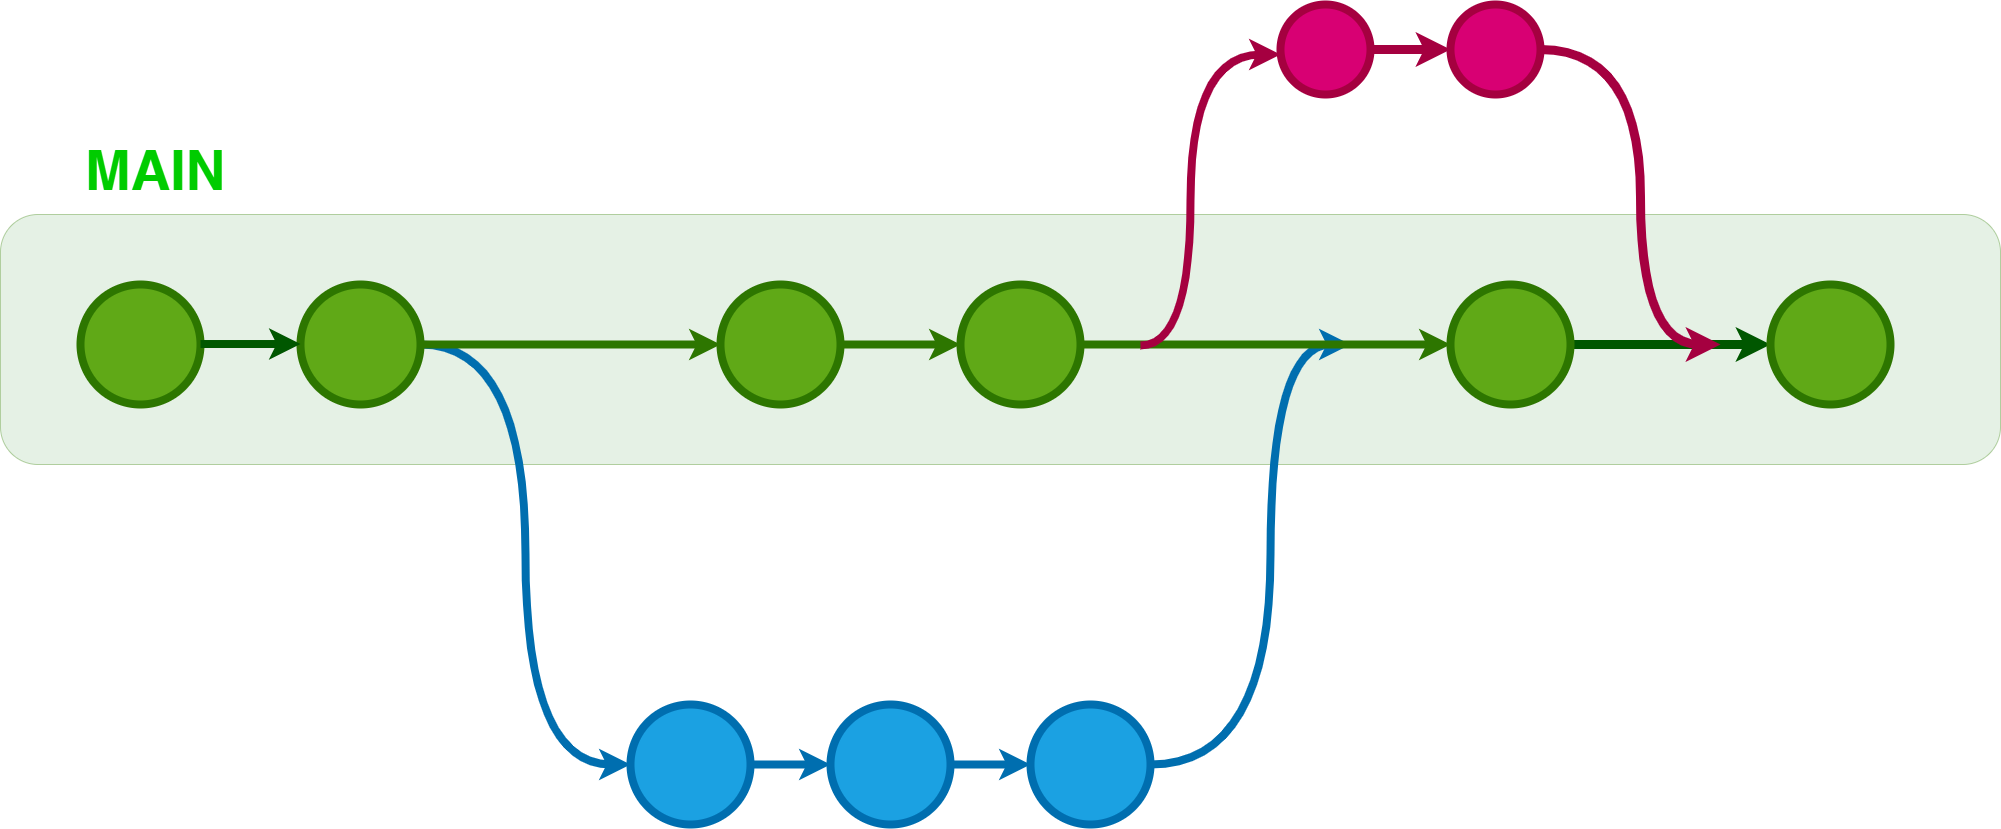
\includegraphics[width=0.7\textwidth]{images/git-branch.png}
     \end{figure}

     \href{https://gitlab.com/blancoapa/pyMBE}{Ejemplo en gitlab}



  \end{frame}

  \begin{frame}
    
    \begin{block}{ Gestión de ramas }
      {\texttt{\$ git branch <nombre\_rama> }}  (Crear)\\
      {\texttt{\$ git branch <nombre\_rama> -d }} (Eliminar) \\
      {\texttt{\$ git switch <nombre\_rama> }} (Cambiar a una rama) \\
      {\texttt{\$ git checkout -b <nombre\_rama> }} (Cambiar a una rama) \\
      {\texttt{\$ git merge }} (Integrar una rama) \\
    \end{block}

    \begin{exampleblock}{git switch vs git checkout }
      \textbf{git switch:} Comando especifico para cambiar entre distintas ramas \\
      \textbf{git checkout:} tiene varias funciones, incluyendo la capacidad de cambiar entre ramas, hash,tags y commits
    \end{exampleblock}

    Ref: Documentación \href{https://docs.github.com/es/pull-requests/collaborating-with-pull-requests/proposing-changes-to-your-work-with-pull-requests/creating-and-deleting-branches-within-your-repository}{git branch} 
  
  \end{frame}

  \begin{frame}{Cambios temporales}
    
    \begin{exampleblock}{Stash}
      Permite guardar temporalmente los cambios que hemos realizado en un archivo, o conjunto de archivos, sin tener que hacer commit
    \end{exampleblock}

    \begin{block}{Reservar cambios}
      {\texttt{\$ git stash}} \\
      {\texttt{\$ git stash list}} \\
      {\texttt{\$ git stash pop}} \\
      {\texttt{\$ git stash drop}} \\
      {\texttt{\$ git stash apply}} \\
      {\texttt{\$ git stash clear}} 
    \end{block}

    Ref: Documentación \href{https://git-scm.com/docs/git-stash}{git stash}
  \end{frame}
  
\begin{frame} {Ignorar Archivos}

  \begin{alertblock}{.gitignore}
    Es un archivo de git que se crea en el repositorio en el cual se esta trabajando.
    Permite ignorar archivos o directorios de los que no deseamos hacer seguimiento.
  \end{alertblock}


    \begin{block}{Creación del archivo .gitignore}
      {\texttt{\$ touch .gitignore }} \\ 
      {\texttt{\$ vim .gitignore }}
    \end{block}

    {Documentación \href{https://docs.github.com/es/get-started/getting-started-with-git/ignoring-files}{.gitignore}}

\end{frame}

\subsection {Sincronización}
  \begin{frame} {\LARGE Sincronización en remoto}
  
      \begin{exampleblock}{Fetch}
        Se utiliza para descargar el historial de cambios del repositorio remoto al repositorio local, pero sin aplicar los cambios.
      \end{exampleblock}
        
      \begin{exampleblock}{Pull}
        Descarga los cambios del repositorio remoto y los fusiona con los cambios locales.
        Si hay conflictos en la fusión git intentara de combinar los cambios por defecto. 
      \end{exampleblock}


      \begin{block}{Comandos de Sincronización}
        {\texttt{\$ git fetch }}  \\
        {\texttt{\$ git config pull.rebase false  }}  \\
        {\texttt{\$ git pull  }}  \\
      \end{block}
    
  \end{frame}

\subsection {Resolución de conflictos} 

  \begin{frame} {Resolución de conflictos}  
    \begin{block}{}
      \texttt{\$ git diff} \\
      \texttt{\$ git diff <hash\_commit\_a> <hash\_commit\_b>}  \\
      \texttt{\$ git reset }  \\
      \texttt{\$ git reset --hard } 
    \end{block}

  
  \end{frame}


\subsection {GitHub funcionalidades}

\begin{frame}{GitHub funcionalidades}

  \begin{itemize}
    \LARGE
    \item Markdown
    \item Issues 
    \item Comentarios
    \item GitHub Pages
  \end{itemize}

\end{frame}


\begin{frame}{GitHub funcionalidades}

  \begin{exampleblock}{Markdown: readme.md}
    Es un archivo que debe incluir una descripción general del proyecto, instrucciones de instalación y configuración. 
    Si es un repositorio publico es recomendable agregar información para constribuir.
    Ejemplo de archivo \href{https://github.com/paobtorres/sistemas_dinamicos_I}{readme.md}
  \end{exampleblock}

  % \begin{figure}[t]
  %   \framezoom<0><2>[border](9cm,0cm)(2cm,1.5cm)
  %   \subfloat[\centering]{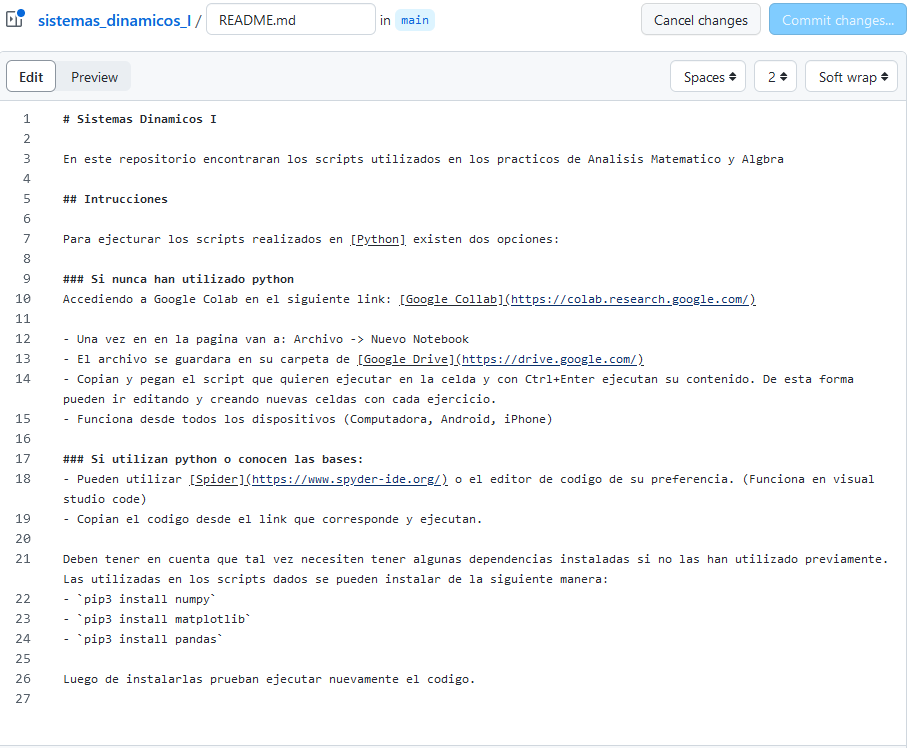
\includegraphics[width=0.15\textwidth]{images/git-readme-md.PNG}}
  %   \subfloat[\centering]{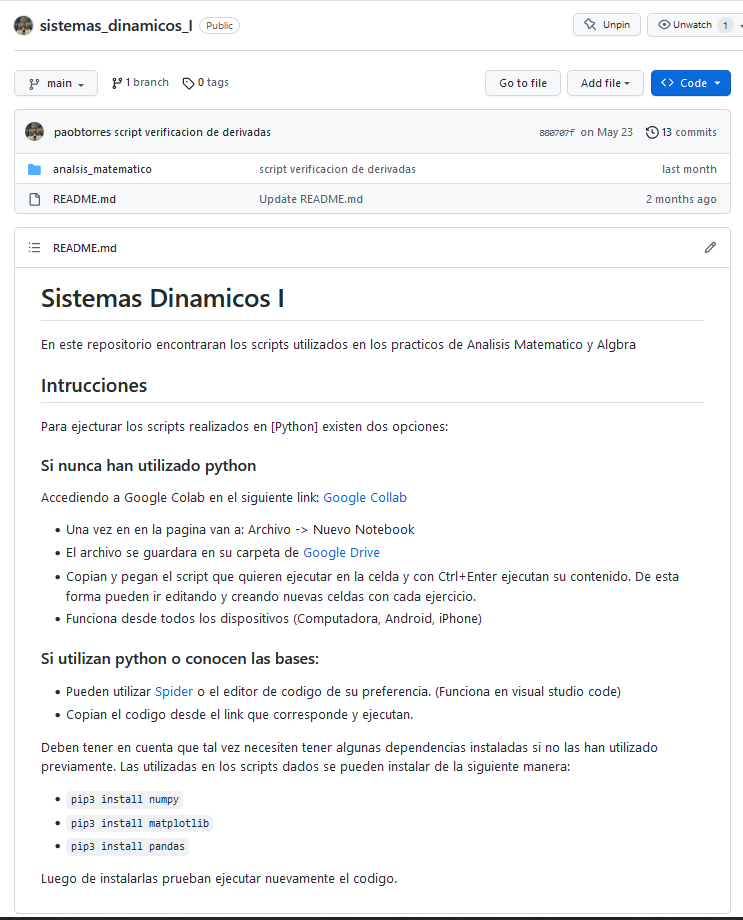
\includegraphics[width=0.15\textwidth]{images/git-readme-preview.PNG}}
  % \end{figure}

  Ref: Documentación \href{https://docs.github.com/es/get-started/writing-on-github/getting-started-with-writing-and-formatting-on-github/quickstart-for-writing-on-github}{markdown}

\end{frame}


\begin{frame}{Issues}
  \begin{figure}
    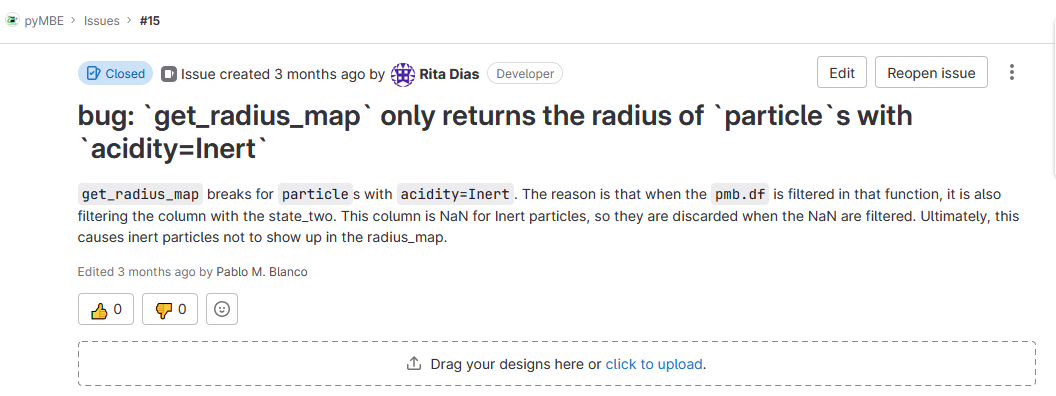
\includegraphics[width=\textwidth]{images/issue.PNG}
  \end{figure}

  \begin{figure}
    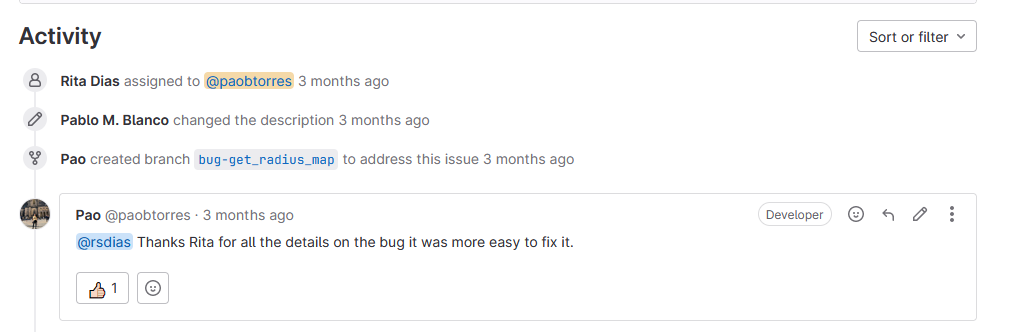
\includegraphics[width=\textwidth]{images/issue-activity.PNG}
  \end{figure}

\end{frame}

\begin{frame} {Herramientas gráficas }
\centering 
    \begin{figure}
      
\includegraphics[width=0.4\textwidth]{images/github-desktop.jpg}
    \end{figure}
    GitHub desktop: \href{https://desktop.github.com/}{Pagina oficial}

    \begin{figure}
      
\includegraphics[width=0.4\textwidth]{images/gitkraken.jpg}
    \end{figure}
    GitKraken: \href{https://www.gitkraken.com/}{Pagina oficial}

    \begin{figure}
      
\includegraphics[width=0.4\textwidth]{images/sourcetree.png}
    \end{figure}

    SourceTree: \href{https://www.sourcetreeapp.com/}{Pagina oficial}


\end{frame}

\subsection {Buenas practicas}
  \begin{frame} {Buenas practicas}
      \begin{itemize}
        \Large
        \item Nombrar los archivos/carpetas/repositorios sin espacios, ni letras como \textbf{ñ} o acentos.
        \item Realizar \texttt{commits} frecuentemente y con indicaciones claras 
        \item Utilizar ramas para desarrollo de tareas especificas
        \item Continuar aprendiendo.
      \end{itemize}
  \end{frame}

  

\section{Referencias}

\begin{frame}{Referencias}

  \begin{itemize}
    \item Documentación oficial de \href{https://git-scm.com}{git} 
    \item Documentación de \href{https://docs.github.com/es}{GitHub} (español)
    \item \href{https://training.github.com/downloads/es_ES/github-git-cheat-sheet/}{cheat-sheet}
  \end{itemize}

\end{frame}

\begin{frame}

\begin{figure}
  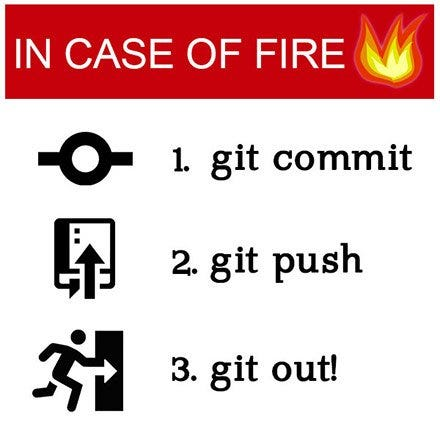
\includegraphics[width = 0.5\textwidth]{images/meme-git.jpg}
\end{figure}

\begin{block}{}
  {\texttt{\$ git add  }} \\
  {\texttt{\$ git commit  }} \\
  {\texttt{\$ git push }}
\end{block}

\end{frame}

\end{document}



% \section*{Contenidos}

% 
% 
% 


% \section*{Prácticas propuestas}
% \begin{itemize}
%     \item Creación de un repositorio local y confirmación de cambios
%     \item Uso de GitHub como herramienta para administrar proyectos. 
%         \item Gestión de repositorios remotos. 
% \item Trabajo con ramas y fusión de ramas
% \item Trabajo colaborativo mediante un repositorio remoto compartido
% \item Control de versiones mediante etiquetado de versiones

% \end{itemize}